\section{Referêncial Teórico}

\subsection{Relação Anual de Informações Sociais (RAIS)}

A gestão governamental do setor do trabalho conta com o importante instrumento de coleta de dados denominado de Relação Anual de Informações Sociais - RAIS (Relação Anual de Informações Sociais) \cite{Sobre_a_RAIS}. Instituída pelo Decreto nº 76.900, de 23 de dezembro de 1975 e regida atualmente pelo Decreto nº 10.854, de 10 de novembro de 2021, a RAIS (Relação Anual de Informações Sociais) tem por objetivo: 

\begin{itemize}
	\item O suprimento às necessidades de controle da atividade trabalhista no País
	\item O provimento de dados para a elaboração de estatísticas do trabalho
	\item A disponibilização de informações do mercado de trabalho às entidades governamentais.
\end{itemize}

\subsection{A pandemia da COVID-19}

::: Artigo - Reforma trabalhista e pandemia -  movimentações contratuais dosas docentes do ensino básico privado de Pernambuco :::

A pandemia da COVID-19 A partir de 2020, se iniciou uma nova crise de proporções globais, provocada pelo coronavírus (Sars-Cov-2). Em 31 de dezembro de 2019, a Organização Mundial de Saúde – OMS foi alertada sobre o surgimento do vírus em Wuhan, na República Popular da China; entendido primeiramente como um caso de pneumonia, posteriormente descobriu-se a existência de um vírus específico. Em 11 de março de 2020, caracterizou-se a pandemia da COVID-19, que provocou milhões de mortes ao redor do mundo. 

Se espalhando em escala global, a doença foi enfrentada de diversas maneiras, a depender da posição política das lideranças governamentais e do alinhamento com medidas sanitárias recomendadas pela OMS. Para evitar o aumento da contaminação, medidas de prevenção foram adotadas, como o uso de equipamentos de proteção individual – EPI, distanciamento e isolamento social. No Brasil, esse processo incluiu uma disputa judicial entre o governo federal e os governos estaduais. O primeiro foi contrário às medidas de isolamento social impostas por estados e municípios, com o argumento da necessidade de proteção da economia e dos empregos. O Supremo Tribunal Federal – STF deu autonomia relativa a estados e municípios e permitiu a ação do governo federal especificamente para reforçar ações protetivas.

O mercado de trabalho, que já apresentava uma constante deterioração de postos desde anos anteriores, viu esse processo tornar-se mais agudo, com aumento das taxas de desocupação (de 12\% no segundo trimestre de 2019 para 13,3\% no segundo semestre de 2020) e subutilização da força de trabalho (de 24,8\% para 29,1\% no mesmo período), além de aumento da informalidade (BRIDI, 2020). 

Em meio ao problema do desemprego, o governo federal publicou duas Medidas Provisórias: a MP 927/2020 e a MP 936/2020 (posteriormente convertida na Lei n. 14.020/2020). A primeira (não mais em vigor) liberou o trabalho remoto, antecipação de férias individuais, coletivas e feriados. Já a segunda, convertida em lei e em vigor, permitiu principalmente (art. 5º) a redução da jornada de trabalho, de salários e a suspensão temporária dos contratos de trabalho, custeados pelo Benefício Emergencial de Preservação do Emprego e da Renda – Bem. Outra medida aprovada e fortemente debatida entre o Congresso e o governo, principalmente quanto ao valor do benefício, foi o Auxílio Emergencial; pela Lei n. 13.982/2020, art. 2º, foram previstas três parcelas de R\$ 600,00 para pessoas em situação de vulnerabilidade3 (o § 3º garantiu o dobro do valor em casos de mulheres provedoras em família monoparental). 

A educação foi fortemente afetada: estudantes e professores/as tiveram de adaptar-se a condições de trabalho remotas, na tentativa de cumprir o programa curricular previsto para o ano letivo. A pandemia em si já era uma situação extraordinária, mas essa migração abrupta, inédita, do regime presencial para o remoto foi seguida por uma série de complicações. Dalila Oliveira e Edmilson Pereira Junior (2020), em pesquisa com professores/as do ensino básico, notaram diferenças grandes nos diferentes níveis da educação em relação ao suporte institucional, condições de acesso a equipamentos para professores/ as e estudantes, sobrecarga de trabalho, mediação do trabalho com atividades domésticas, além do aumento de esforço para atrair a atenção de estudantes.

\subsection{Cross Industry Standard Process for Data Mining (CRISP-DM)}

::: Artigo - Deep Learning Anomaly Detection as Support Fraud Investigation in Brazilian Exports and Anti-Money Laundering :::

This study used as reference model the Cross Industry Standard Process for Data Mining (CRISP-DM) \cite{chapman2000crisp}, since it is a well-known data mining reference model. The CRISPDM methodology is flexible and allows the creation of a model that fits the specific needs of projects. It is observed that the execution sequence of the phases is not rigid and depends on the results achieved in each phase (see Figure \ref{fig1}).

\begin{figure}[htbp]
	\centerline{
		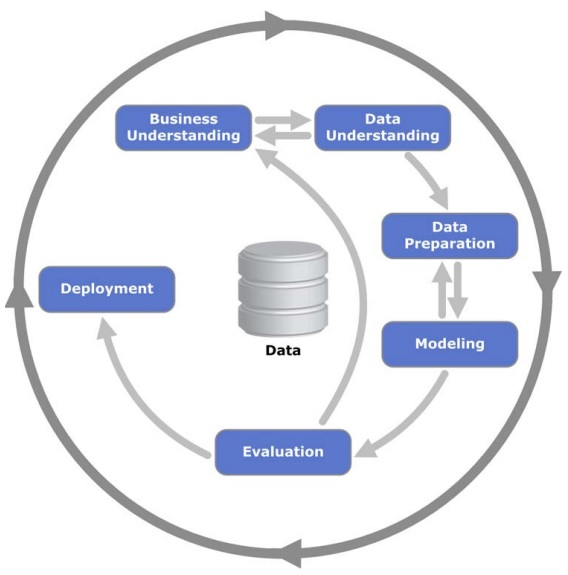
\includegraphics[width=80mm,scale=0.8]{assets/crispdm.jpg}
	}
	\caption{Phases of the CRISP-DM Process Model}
	\label{fig1}
\end{figure}

The life cycle of the mining project on this methodology consists of six phases: 

\begin{itemize}
	\item Business understanding This initial phase focuses on understanding the goals and project requirements from a business perspective, then converting that knowledge into a definition of the data mining problem and a preliminary plan designed to achieve the objectives. 
	      	      	      	      	      	      	      	      
	      	      	      	      	      	      	      	        
	\item Data understanding The data understanding phase starts with the initial data collection and continues with activities that allow the familiarization with the data, the identification of data quality problems, the discovery of the first insights into the data and/or detection of interesting subsets to form hypotheses about the unknown information. Sections 1 and 4 of this paper summarize the results of this step of the methodology. 
	      	      	      	      	      	      	      	      
	\item Data preparation The data preparation phase concentrates all activities necessary to the construction of the final data set to be used in the modeling phase. Data preparation tasks are typically performed several times and not in any prescribed order. The tasks include selecting, cleaning, constructing, integrating and formatting data for modeling purposes. 
	      	      	      	      	      	      	      	      
	\item Modeling At this stage, several modelling techniques are chosen and applied and its parameters are adjusted to the optimum values. Usually, there are many different techniques for the same data mining problem. Some techniques have specific requirements regarding the form of the data. Thus, it is often necessary to go back to previous phases to perform adjustments. 
	      	      	      	      	      	      	      	      
	\item Evaluation In this phase, it is important to evaluate and review the steps performed to create the final model (or models), before final deployment, to make sure it achieves the business objectives. It is important to try to determine if there are any important business issues not yet considered. At the end of this phase, it is important to decide if the results are satisfactory and whether the final model should be used or not. 
	      	      	      	      	      	      	      	      
	\item Deployment The knowledge obtained with the models generated must be applied in the Organization and this knowledge must be disseminated and presented to users in a way that they can use it.
	      	      	      	      	      	      	      	      
\end{itemize}